\RequirePackage{plautopatch}
\documentclass[13pt,aspectratio=169,table,dvipdfmx]{beamer}

\usepackage{animate}
\usepackage{bxdpx-beamer}
\usepackage{amsmath, amssymb, amsthm, mathrsfs, amsfonts, dsfont}
\usepackage[ruled, vlined]{algorithm2e}
\usepackage{annotate-equations}
\usepackage{bbm}
\usepackage{bm}
\usepackage{booktabs}
\usepackage{breakcites}
\usepackage{calc}
\usepackage[style=base]{caption}
\usepackage{enumerate}
\usepackage[T1]{fontenc}
\usepackage{ifthen}
\usepackage{listings}
\usepackage{mathtools}
\usepackage{mlmodern}
\usepackage{multirow}
\usepackage{newtxtext}
\usepackage{optidef}
\usepackage[deluxe]{otf}
\usepackage{physics}
\usepackage{setspace}
\usepackage{stfloats}
\usepackage{subfiles}
\usepackage{subcaption}
\usepackage{svg}
\usepackage{tikz}
\usepackage{xparse}
\usepackage[all]{xy}

% === Commands ===

\definecolor{cA}{HTML}{0072BD}
\definecolor{cB}{HTML}{EDB120}
\definecolor{cC}{HTML}{77AC30}
\definecolor{cD}{HTML}{D95319}
\definecolor{cE}{HTML}{7E2F8E}
\newcommand{\red}[1]{\textcolor{red}{#1}}
\newcommand{\blue}[1]{\textcolor{blue}{#1}}
\newcommand{\cyan}[1]{\textcolor{cyan}{#1}}
\newcommand{\gray}[1]{\textcolor{gray}{#1}}
\newcommand{\green}[1]{\textcolor{green}{#1}}
\newcommand{\brown}[1]{\textcolor{brown}{#1}}
\newcommand{\black}[1]{\textcolor{black}{#1}}
\newcommand{\orange}[1]{\textcolor{orange}{#1}}
\newcommand{\purple}[1]{\textcolor{purple}{#1}}
\newcommand{\yellow}[1]{\textcolor{yellow}{#1}}
\newcommand{\Magenta}[1]{\textcolor{Magenta}{#1}}
\newcommand{\RoyalBlue}[1]{\textcolor{RoyalBlue}{#1}}
\newcommand{\RubineRed}[1]{\textcolor{RubineRed}{#1}}
\newcommand{\ForestGreen}[1]{\textcolor{ForestGreen}{#1}}
\newcommand{\YellowOrange}[1]{\textcolor{YellowOrange}{#1}}
\newcommand{\WildStrawberry}[1]{\textcolor{WildStrawberry}{#1}}
\newcommand{\cAText}[1]{\textcolor{cA}{#1}}
\newcommand{\cBText}[1]{\textcolor{cB}{#1}}
\newcommand{\cCText}[1]{\textcolor{cC}{#1}}
\newcommand{\cDText}[1]{\textcolor{cD}{#1}}

\newcommand{\st}{\text{ s.t. }}
\newcommand{\Img}[1]{\mathrm{Im}\qty(#1)}
\newcommand{\Ker}[1]{\mathrm{Ker}\qty(#1)}
\newcommand{\Supp}[1]{\mathrm{supp}\qty(#1)}
\newcommand{\Rank}[1]{\mathrm{rank}\qty(#1)}
\newcommand{\floor}[1]{\left\lfloor #1 \right\rfloor}
\newcommand{\ceil}[1]{\left\lceil #1 \right\rceil}
% C++ (https://tex.stackexchange.com/questions/4302/prettiest-way-to-typeset-c-cplusplus)
\newcommand{\Cpp}{C\nolinebreak[4]\hspace{-.05em}\raisebox{.4ex}{\relsize{-3}{\textbf{++}}}}
% https://tex.stackexchange.com/questions/28836/typesetting-the-define-equals-symbol
\newcommand{\defeq}{\coloneqq}
\newcommand{\eqdef}{\eqqcolon}
% https://tex.stackexchange.com/questions/5502/how-to-get-a-mid-binary-relation-that-grows
\newcommand{\relmiddle}[1]{\mathrel{}\middle#1\mathrel{}}

\DeclareMathOperator{\Proj}{Proj}
\DeclareMathOperator{\Exp}{Exp}
\DeclareMathOperator{\Hess}{Hess}
\DeclareMathOperator{\Retr}{Retr}
\DeclareMathOperator{\Span}{span}
\DeclareMathOperator{\myGrad}{grad}
\renewcommand{\grad}{\myGrad}

% https://tex.stackexchange.com/questions/564216/newcommand-for-each-letter
\ExplSyntaxOn
\NewDocumentCommand{\definealphabet}{mmmm}{
\int_step_inline:nnn{`#3}{`#4}{
\cs_new_protected:cpx{#1 \char_generate:nn{##1}{11}}{
\exp_not:N #2{\char_generate:nn{##1}{11}}}}}
\ExplSyntaxOff

\definealphabet{bb}{\mathbb}{A}{Z}
\definealphabet{rm}{\mathrm}{A}{Z}
\definealphabet{cal}{\mathcal}{A}{Z}
% \definealphabet{scr}{\mathscr}{A}{Z}
\definealphabet{frak}{\mathfrak}{a}{z}
\definealphabet{frak}{\mathfrak}{A}{Z}

% === Settings ===

% https://qiita.com/rityo_masu/items/efd44bc8f9229e014237
\allowdisplaybreaks[4]

\usetikzlibrary{
  3d,
  fit,
  calc,
  math,
  matrix,
  patterns,
  backgrounds,
  arrows.meta,
  decorations.pathmorphing,
}

% This declares a command \Comment
% The argument will be surrounded by /* ... */
% https://ja.overleaf.com/learn/latex/Algorithms
\SetKwComment{Comment}{/* }{ */}

\DontPrintSemicolon

\parindent=0pt

% === Beamer Settings ===

\usetheme{Boadilla}

\usefonttheme{professionalfonts} % Be professional!

% https://tex.stackexchange.com/questions/646333/size-of-integral-symbol-in-section-header-with-mlmodern
\DeclareFontFamily{OMX}{mlmex}{}
\DeclareFontShape{OMX}{mlmex}{m}{n}{%
   <->mlmex10%
   }{} 
\renewcommand{\familydefault}{\sfdefault}
\usefonttheme{structurebold}
\setbeamerfont{alerted text}{series=\bfseries}
\setbeamerfont{section in toc}{series=\mdseries}
\setbeamerfont{itemize/enumerate body}{size=\large}

%Beamer Color
\definecolor{blendedblue}{rgb}{0.2,0.2,0.7}
\definecolor{UniBlue}{RGB}{0,150,200} 
\definecolor{UniGreen}{RGB}{0,200,150}
\definecolor{AlertOrange}{RGB}{255,76,0}
\definecolor{AlmostBlack}{RGB}{38,38,38}
\setbeamercolor{normal text}{fg=AlmostBlack}
\setbeamercolor{structure}{fg=UniBlue}
\setbeamercolor{block title}{fg=UniBlue!50!black}
\setbeamercolor{alerted text}{fg=AlertOrange}
\setbeamercolor{itemize item}{fg=black}
\setbeamercolor{itemize subitem}{fg=black}
\setbeamercolor{itemize subsubitem}{fg=black}

\setbeamertemplate{blocks}[rounded]
\useinnertheme{circles}
\setbeamertemplate{navigation symbols}{}
\setbeamertemplate{footline}[page number]

\setbeamertemplate{title page}{%
    \vspace{2.5em}
    {\usebeamerfont{title} \usebeamercolor[fg]{title} \inserttitle \par}
    {\usebeamerfont{subtitle}\usebeamercolor[fg]{subtitle}\insertsubtitle \par}
    \vspace{1.5em}
    \begin{flushright}
        \usebeamerfont{author}\insertauthor\par
        \usebeamerfont{institute}\insertinstitute \par
        \vspace{3em}
        \usebeamerfont{date}\insertdate\par
        \usebeamercolor[fg]{titlegraphic}\inserttitlegraphic
    \end{flushright}
}

% === TITLE ===
\title{\Huge{Improved Initial Placement for\\Fruchterman--Reingold Algorithm}}
\author{\Large{Hiroki Hamaguchi}}
\institute{\large{Supervisors: Prof. Akiko Takeda\\\phantom{Supervisors: }Pierre-Louis Poirion\\\phantom{Supervisors: }Andi Han}\\\phantom{Supervisors: }if ok, Prof. Naoki Marumo}
\date{2024/06/17}

\newif\ifShowHidden
\ShowHiddenfalse
% \ShowHiddentrue

\begin{document}

\ifShowHidden
    \maketitle
\fi

\ifShowHidden
    \begin{frame}{Introduction for Graph Drawing}
        \begin{tikzpicture}
            \node[cA,font=\bfseries] (A) at (0,0) {Graph Drawing};
            \node[cB,font=\bfseries] (B) at (-3.0,-1) {Discrete Based};
            \node[align=left,anchor=north west] (B1) at ($(B)+(-2.0,-0.6-0.0)$) {\textcolor{cB}{BFS layout}\\\small{\quad - for tree graph}};
            \node[align=left,anchor=north west] (B2) at ($(B)+(-2.0,-0.6-1.0)$) {\textcolor{cB}{Planar layout}\\\small{\quad - for planar graph}\\\scriptsize{\quad - \cite{tutteHowDrawGraph1963}}\\\scriptsize{\quad - \cite{chrobakLineartimeAlgorithmDrawing1995}}};
            \node[align=left,anchor=north west] (B3) at ($(B)+(-2.0,-0.6-3.0)$) {\textcolor{cB}{Layered graph drawing}\\\small{\quad - for DAG}\\\scriptsize{\quad - \cite{sugiyamaMethodsVisualUnderstanding1981}}};
            \node[align=left,anchor=north west] (B4) at ($(B)+(-2.0,-0.6-4.5)$) {\textcolor{cB}{Spectral layout~}\\\small{\quad - eigenvector of Laplacian}};
            \node[draw=cB, thick,fit={(B1) (B2) (B3) (B4)}, inner sep=5pt] (BBox) {};

            \node[cC,font=\bfseries] (C) at (+4.5,-1) {Continuous Based};
            \node[cC,font=\bfseries] (C1) at ($(C)+(-2.5,-1)$) {Kamada--Kawai (KK)};
            \node[cC,font=\bfseries] (C11) at ($(C1)+(0,-0.5)$) {\scriptsize{\cite{kamadaAlgorithmDrawingGeneral1989}}};
            \node at ($(C11)+(0,-1.0)$) {
                \begin{minipage}{4cm}
                    \begin{gather*}
                        \mathrm{minimize}\\
                        \sum_{i < j} \frac{k_{i,j}}{2} (d_{i,j}-l_{i,j})^2
                    \end{gather*}
                \end{minipage}
            };
            \node[cC,font=\bfseries] (C2) at ($(C)+(+2.5,-1)$) {Fruchterman--Reingold (FR)};
            \node[cC,font=\bfseries,align=center] (C21) at ($(C2)+(0,-0.5)$) {\scriptsize{\cite{fruchtermanGraphDrawingForcedirected1991}}};
            \node at ($(C21)+(0,-1.0)$) {
                \begin{minipage}{4cm}
                    \begin{gather*}
                        \mathrm{minimize}\\
                        \sum_{i<j} \qty(\frac{a_{i,j} d_{i,j}^3}{3k} - k^2\log{d_{i,j}})
                    \end{gather*}
                \end{minipage}
            };

            \node[align=center] (C3) at ($(C)+(0.5,-4.3)$) {
            \scriptsize{$d_{i,j}$: distance between nodes $v_i,v_j$ / $l_{i,j}$: optimal distance / $k,a_{i,j}$: constant}
            };

            \node (C01) at ($(C)+(-3.5,-5.5)$) {
                
\includegraphics[width=1cm]{imgs/networkx_logo.png}
            };
            \node (C02) at ($(C)+(-2.5,-5.5)$) {
                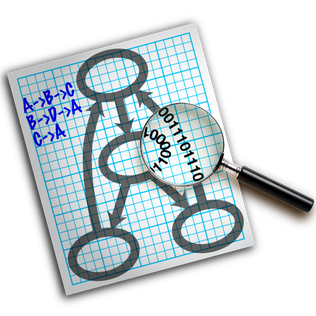
\includegraphics[width=1cm]{imgs/GraphvizLogo.png}
            };
            \node[anchor=west] (C03) at ($(C)+(-2,-5.5)$) {
                NetworkX and Graphviz support KK and FR
            };
            \node[draw=cC, thick,fit={(C01) (C02) (C03)}, inner sep=5pt] (CBox) {};

            \draw[thick,->] (A) |- ($(A)!0.5!(B)$) -| (B);
            \draw[thick,->] (A) |- ($(A)!0.5!(C)$) -| (C);
            \draw[thick,->] (C) |- ($(C)!0.5!(C1)$) -| (C1);
            \draw[thick,->] (C) |- ($(C)!0.5!(C2)$) -| (C2);
        \end{tikzpicture}
    \end{frame}
\fi

\ifShowHidden
    \begin{frame}{Definition of FR Layout}
        \begin{itemize}
            \item Historically, FR layout seeks an equilibrium of two forces:
        \end{itemize}
        \begin{equation*}
            F_{i,j}^a(d) \defeq \frac{a_{i,j} d^2}{k} \text{\quad (attraction)}, \quad F^r(d) \defeq -\frac{k^2}{d} \text{\quad (repulsion)}
        \end{equation*}
        \begin{itemize}
            \item This problem can be redefine as an optimization problem:
        \end{itemize}
        \begin{equation*}
            \mathrm{minimize} \sum_{i<j} E_{i,j}(d)
            \quad \mathrm{where} \quad
            E_{i,j}(d) \defeq \int_{0}^{d} F_{i,j}^a(r) \dd{r} + \int_{\infty}^{d} F^r(r) \dd{r} = \frac{a_{i,j} d^3}{3k} - k^2\log{d}
        \end{equation*}
        \begin{figure}[htbp]
            \begin{minipage}{0.49\hsize}
                \centering
                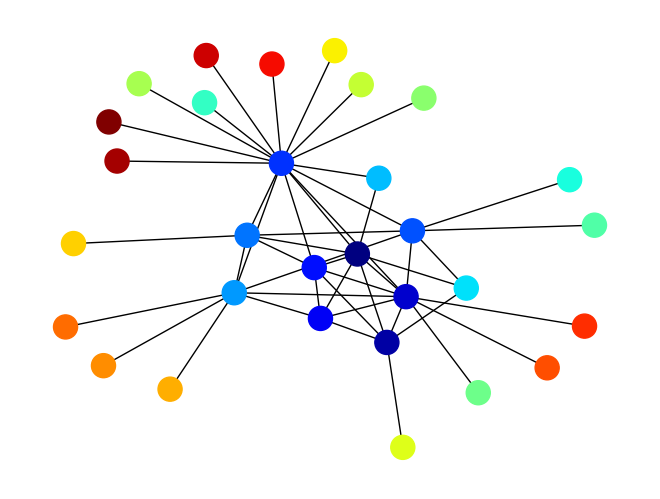
\includegraphics[width=0.6\columnwidth]{imgs/example_fr.png}
                \caption{Example of FR layout}
            \end{minipage}
            \begin{minipage}{0.49\hsize}
                \centering
                \begin{tikzpicture}
                    \def\yAdjust{2}
                    \def\d{4}
                    \def\r{0.3}
                    \def\u{1.0}
                    \coordinate (M1) at (0,0);
                    \coordinate (M2) at (\d,0);

                    \draw (M1) circle(\r) node {$v_i$};
                    \draw (M2) circle(\r) node {$v_j$};

                    \draw (0,+1.6*\r*\yAdjust) -- (0,+2.4*\r*\yAdjust);
                    \draw (\d,+1.6*\r*\yAdjust) -- (\d,+2.4*\r*\yAdjust);
                    \draw[{Latex[length=4,width=3]}-{Latex[length=4,width=3]}] ($(M1)+(90:2*\r*\yAdjust)$) -- ($(M2)+(90:2*\r*\yAdjust)$)
                    node[midway,circle,fill=white,inner sep=0] {$d$};

                    \draw[->,thick,line cap=round] (+\r,0) -- (+\u,0) node[right] {$F^a_{i,j}(d)$};
                    \draw[->,thick,line cap=round] (-\r,0) -- (-\u,0) node[left] {$F^r(d)$};

                    \draw[dashed,domain=3.9:-3.1,samples=1000,smooth,variable=\x] plot(\x,{(-0.7+(pow((\d-\x)/\d,3)/3-ln((\d-\x)/\d))/2.2)*\yAdjust});
                    \node [star,
                        minimum size=0.25cm,
                        star point ratio=2.25,
                        inner sep=0pt,
                        draw, fill=black]
                    at (0,{(-0.7+(1/3)/2.2)*\yAdjust}) {};

                    \node at (-2.7,0.4*\yAdjust) {$E_{i,j}(d)$};
                \end{tikzpicture}
            \end{minipage}
        \end{figure}
    \end{frame}
\fi

\ifShowHidden
    \begin{frame}{Algorithm for FR Layout 1}
        \begin{columns}
            \begin{column}{0.4\columnwidth}
                \textbf{``spring\_layout'' in NetworkX}
                \begin{itemize}
                    \item Adaptive cooling scheme
                    \item \textbf{gradient descent method}\\with constant step size\\per each vertex
                    \item \cite{tunkelang1999numerical}
                    \item strong \textbf{theoretical background}
                \end{itemize}
            \end{column}
            \begin{column}{0.6\columnwidth}
                \begin{figure}[htbp]
                    \centering
                    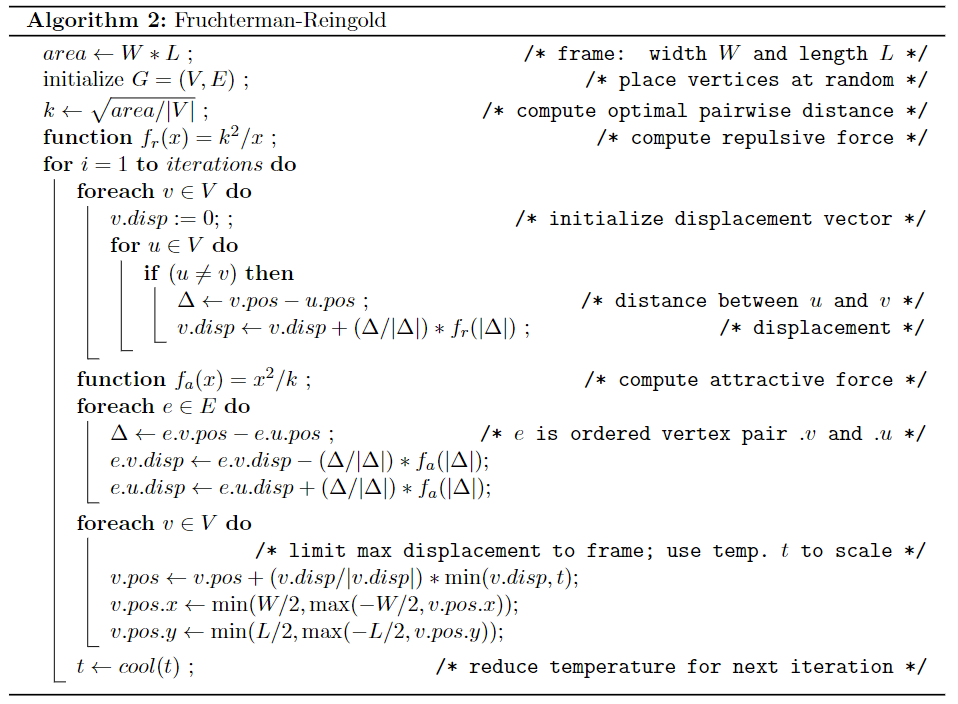
\includegraphics[width=\columnwidth]{imgs/FR_code.png}
                    \caption{\cite{kobourov2012spring}}
                \end{figure}
            \end{column}
        \end{columns}
    \end{frame}
    \begin{frame}{Algotithm for FR Layout 2}
        \begin{columns}
            \begin{column}{0.4\columnwidth}
                \textbf{``sfdp'' in Graphviz}
                \begin{itemize}
                    \item Scalable Force-Directed Placement
                    \item \textbf{Multilevel} approach
                    \item Barnes--Hat algorithm (Q-tree)\cite{Hu2006EfficientHF}
                          \cite{barnesHierarchicalLogForcecalculation1986}
                    \item These methods are\\\textbf{out of scope},\\
                          but our work is still applicable.
                \end{itemize}
            \end{column}
            \begin{column}{0.6\columnwidth}
                \begin{figure}[htbp]
                    \centering
                    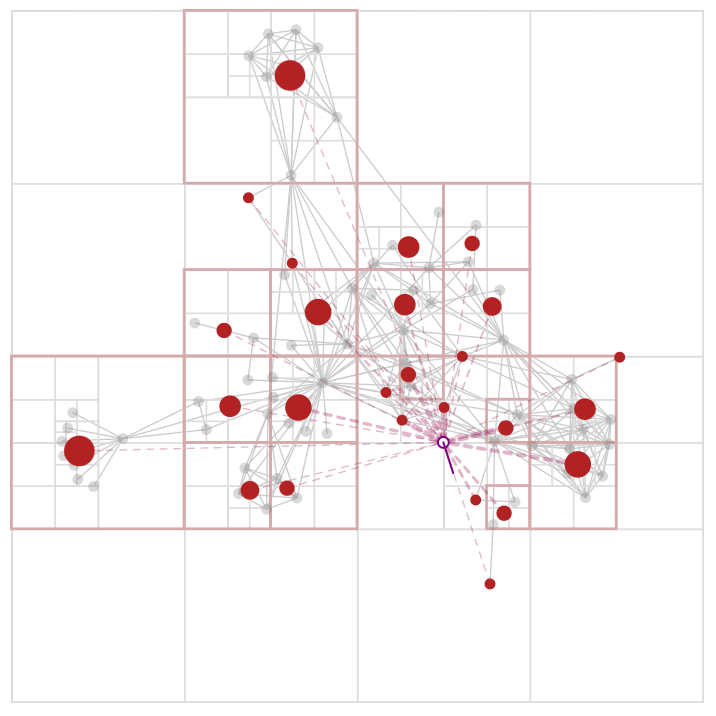
\includegraphics[width=0.7\columnwidth]{imgs/BH.png}
                    \caption{\footnotesize{\url{https://jheer.github.io/barnes-hut/}}}
                \end{figure}
            \end{column}
        \end{columns}
    \end{frame}
\fi

\ifShowHidden
    \begin{frame}{Hardness of graph drawing}
        \begin{itemize}
            \item Drawing $\bigcirc$ $\cong$ untangling tangled earphones
            \item Escaping from a plateau is very difficult
        \end{itemize}
        \begin{figure}[htbp]
            \begin{minipage}{0.59\hsize}
                \centering
                % \animategraphics[autoplay,loop,width=0.8\columnwidth]{5}{imgs/circle/circle-}{1}{50}
                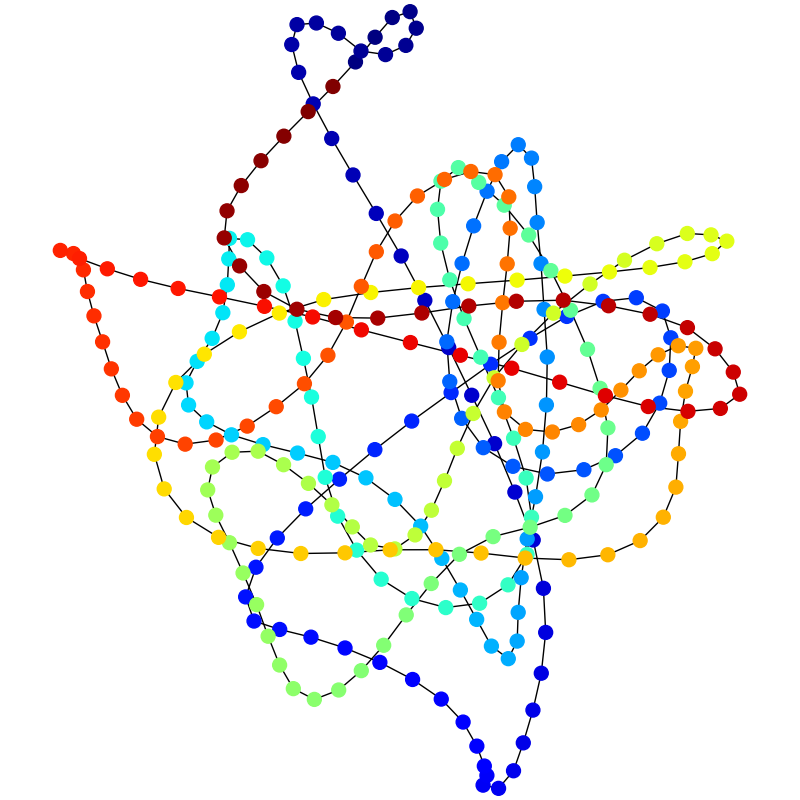
\includegraphics[width=0.8\columnwidth]{imgs/circle/circle-50.png}
                \caption{FR layout by NetworkX}
            \end{minipage}
            \begin{minipage}{0.40\hsize}
                \centering
                \includesvg[width=0.8\columnwidth]{imgs/circle_fdp.svg}
                \caption{fdp layout by Graphviz}
            \end{minipage}
        \end{figure}
    \end{frame}
\fi

\ifShowHidden
    \begin{frame}{Graph Drawing as Continuous Optimization Problem}
        \begin{itemize}
            \item Research on graph drawing by \textbf{continuous optimization} is a hot topic.
                  \begin{itemize}
                      \large{
                      \item stress majorization \cite{gansnerGraphDrawingStress2005}
                      \item \textbf{L-BFGS} method~\cite{6183577} \textcolor{cE}{(8 cites)}
                      \item GPU based \cite{gajdosParallelFruchtermanReingold2016}
                      \item \textbf{SGD} (stochastic gradient descent)~\cite{8419285} \textcolor{cE}{(66 cites)}
                      \item and so on \cite{ahmedGraphDrawingGradient2020,ahmedMulticriteriaScalableGraph2022}
                            }
                  \end{itemize}
        \end{itemize}
        $\to$ Our research aims to take over this flow of the research.
    \end{frame}
\fi

\ifShowHidden
    \begin{frame}{Problem: Inapplicability of SGD}
        \begin{columns}
            \begin{column}{0.1\columnwidth}\end{column}
            \begin{column}{0.4\columnwidth}
                \begin{equation*}
                    \mathrm{(KK)} \quad  f_{i,j}(d) = \frac{k}{2} (d_{i,j} - l_{i,j})^2
                \end{equation*}
            \end{column}
            \begin{column}{0.4\columnwidth}
                \begin{equation*}
                    \mathrm{(FR)} \quad  f_{i,j}(d) = \frac{a_{i,j} d^3}{3k} - k^2\log{d}
                \end{equation*}
            \end{column}
            \begin{column}{0.1\columnwidth}\end{column}
        \end{columns}
        \begin{figure}[htbp]
            \centering
            \begin{tikzpicture}
                \def\radius{2}
                \foreach \xShift/\nA/\nB/\nC/\nD/\nE/\nF/\desc in {
                        -3/1/2/3/3/2/1/$l_{i,j}$,
                        +3/1/0/0/0/0/1/$a_{i,j}$} {
                        \begin{scope}[xshift=\xShift cm]
                            \node at (-0.85*\radius,+0.85*\radius) {\large{\desc}};
                            \node (P0) at (0:\radius) [circle, fill=red, inner sep=0pt, minimum size=10pt] {};
                            \foreach \i in {1,...,6} {
                                    \node (P\i) at (\i*360/7: \radius) [circle, fill=black, inner sep=0pt, minimum size=6pt] {};
                                }
                            \draw (P0) -- (P1) -- (P2) -- (P3) -- (P4) -- (P5) -- (P6) -- (P0);
                            \foreach \i in {1,...,6} {
                                    \draw [decorate, decoration={coil,aspect=0.6,segment length=2mm,amplitude=1mm}] (P\i) -- (P0);
                                }
                            \node[right=5pt] at ($(P0)!0.5!(P1)$) {\nA};
                            \node[above=5pt] at ($(P0)!0.5!(P2)$) {\nB};
                            \node[above=5pt] at ($(P0)!0.5!(P3)$) {\nC};
                            \node[below=5pt] at ($(P0)!0.5!(P4)$) {\nD};
                            \node[below=5pt] at ($(P0)!0.5!(P5)$) {\nE};
                            \node[right=5pt] at ($(P0)!0.5!(P6)$) {\nF};
                        \end{scope}
                    }
            \end{tikzpicture}
        \end{figure}
        \begin{itemize}
            \item KK layout first computes the optimal distance $l_{i,j}$ by Dijkstra's algorithm.
            \item FR layout has $a_{i,j}=0$ if $v_i,v_j$ are not connected.
            \item Can we make a variant of SGD for FR layout?
        \end{itemize}
    \end{frame}
    \begin{frame}{余談用}
        Graph Drawing by Stochastic Gradient Descent
        Jonathan X. Zheng, Samraat Pawar, Dan F. M. Goodman
        からの抜粋:

        \begin{center}
            \begin{tikzpicture}
                \draw (0,0) -- (10,0);
            \end{tikzpicture}
        \end{center}

        このアイデアにはいくつかの問題があります。
        ひとつは、すべての長距離の力を同等に扱うことが、グラフ理論上の距離に忠実でないという点です。
        もうひとつは、これらの力の相対的な強さが、グラフの最終的な配置に大きな影響を与える可能性のある追加パラメータに依存しているという点です【23】。
        これをグラフ理論上の距離に依存させ続ければ、これらの問題を回避することができますが、最短経路の計算と保存の問題が再び発生します。
        この依存関係を維持するためのアプローチのひとつとして、Khoury らによるものがあります【21】。
        彼らは、特異値分解に基づく距離行列の低ランク近似を用いています。
        これにより非常に高い効果が期待できますが、それでもAPSP(全対最短経路問題)を必要とします。
    \end{frame}
\fi

% \ifShowHidden
\begin{frame}{The Purpose of this research}
    \begin{table}
        \centering
        \begin{tabular}{c|c|c|c}
            \toprule
            Existing works      & A                        & B                         & C                    \\
            \midrule
            \textbf{abst}       & L-BFGS for graph drawing & SGD for graph drawing     & SA for graph drawing \\
            \textbf{What we do} & practical speed up       & counterpart for FR layout & refine the strategy  \\
            \bottomrule
        \end{tabular}
    \end{table}
\end{frame}
% \fi

\ifShowHidden
    \begin{frame}{\LARGE{余談: 試した手法群}}
        \begin{itemize}
            \item シンプルなrandom subspace algorithm
            \item (丸茂先生のアドバイスにもあった) 頂点毎にL-BFGSを適用
                  \begin{itemize}
                      \item (cubic regularized Newton以前の問題)
                  \end{itemize}
            \item CG法
            \item stochastic CG法 ``Stochastic Conjugate Gradient Algorithm with
                  Variance Reduction''
            \item L-BFGS法自体の改良の検討 -> 自作だと数値爆発で諦め
            \item 汎用的なフレームワークの開発はこの時点で大分諦めました
        \end{itemize}
    \end{frame}
\fi

% \begin{frame}{Key Technique 1: Separation of the objective function}
%     \begin{itemize}
%         \item SA based close
%         \item
%     \end{itemize}
% \end{frame}

% \begin{frame}{Key Observation: stochastic strategy}
%     \begin{tikzpicture}
%         % Define positions for the first cluster (left)
%         \foreach \xA/\yA/\xB/\yB/\xC/\yC/\xD/\yD/\xE/\yE/\xShift/\yShift in {
%                 0/0/0/1/0/-1/1/0/-1/0/0/0,
%                 0/0/0/1/0/-1/1/0/-1/0/5/2,
%                 0/0/0/1/0/-1/1/0/-1/0/9/2,
%                 0/0/0/1/0/-1/1/0/-1/0/5/-2,
%                 0/0/0/1/0/-1/1/0/-1/0/9/-2} {
%                 \begin{scope}[xshift=\xShift cm,yshift=\yShift cm]
%                     \draw[dashed,color=gray,line width=0.5pt] (-1.5, 1.5) rectangle (1.5, -1.5);
%                     \node[circle, fill=red,   minimum size=8pt] (a0) at (\xA, \yA) {};
%                     \node[circle, fill=black, minimum size=8pt] (a1) at (\xB, \yB) {};
%                     \node[circle, fill=black, minimum size=8pt] (a2) at (\xC, \yC) {};
%                     \node[circle, fill=black, minimum size=8pt] (a3) at (\xD, \yD) {};
%                     \node[circle, fill=black, minimum size=8pt] (a4) at (\xE, \yE) {};
%                     \draw[decorate, decoration={coil, segment length=2, aspect=0.5}] (a0) -- (a1);
%                     \draw[decorate, decoration={coil, segment length=2, aspect=0.5}] (a0) -- (a2);
%                     \draw[decorate, decoration={coil, segment length=2, aspect=0.5}] (a0) -- (a3);
%                     \draw[decorate, decoration={coil, segment length=2, aspect=0.5}] (a0) -- (a4);
%                 \end{scope}
%             }

%         % \node at (0, -1.5) {others are incorrect};
%         % \node at (5, -3.5) {others are incorrect};

%     \end{tikzpicture}
% \end{frame}

% \begin{frame}{key technique}
%     \begin{itemize}
%         \item random subspace algorithm
%               \begin{itemize}
%                   \item \cite{cartisRandomisedSubspaceMethods2022},\cite{fujiRandomizedSubspaceRegularized2022},
%               \end{itemize}
%     \end{itemize}
% \end{frame}

% \ifShowHidden
%     \begin{frame}{Possible Application 1}
%         \begin{figure}[htbp]
%             \centering
%             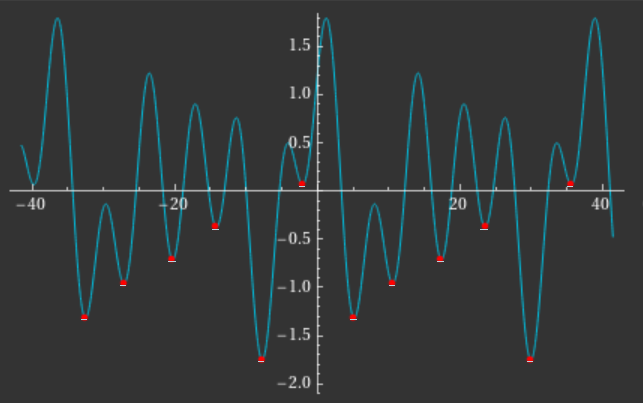
\includegraphics[width=0.5\columnwidth]{imgs/applicatoin1d.png}
%         \end{figure}
%         \begin{itemize}
%             \item Optimize $f(x)$ where $x \in \mathbb{R}^{n}$.
%             \item If two of the points are too close, $f(x)$ drastically increases.
%             \item Similar algorithms might be applicable to this problem.
%             \item Is there any concrete instance?
%             \item Is there any algorithm already well known?
%         \end{itemize}
%     \end{frame}
%     \begin{frame}{Possible Application 2}
%         \begin{itemize}
%             \item (Continuous relaxation of) graph isomorphism problem
%                   \begin{itemize}
%                       \item displaying symmetry is at least as difficult as graph isomorphism \cite{eades1984heuristic}
%                       \item When we draw $G \defeq G_1 \cup G_2$, $G$ displays symmetry if $G_1 \cong G_2$.
%                   \end{itemize}
%             \item Graph isomorphism problem with Frank-Wolfe algorithm \cite{klusContinuousOptimizationMethods2023}
%                   \begin{mini*}
%                       {Q}{||QA-BQ||^2_F}{}{}
%                       \addConstraint{Q}{\in \left\{ Q \in \mathbb{R}^{n \times n} \relmiddle| Q^\top Q = I_n \right\}}
%                   \end{mini*}
%             \item Many-to-Many graph isomorphism \cite{zaslavskiyManytoManyGraphMatching2010}
%                   \begin{mini*}
%                       {P}{||G - PHP^\top ||^2_F}{}{}
%                       \addConstraint{P}{\in \left\{ P \in \{0, 1\}^{n \times n} \relmiddle| P1_n = 1_n, P^\top 1_n = 1_n \right\}}
%                   \end{mini*}
%             \item I'm still doubtful, but these papers seems really interesting. (+ Riemannian optimization)
%         \end{itemize}
%     \end{frame}
% \fi

\setbeamercolor{structure}{fg=blendedblue}
\setbeamercolor{block title}{fg=blendedblue!50!black}

\ifShowHidden
    \begin{frame}{\LARGE{Summary}}
        \begin{block}{Future Work}
            \begin{itemize}
                \item More numerical experiments
                \item Theoretical analysis
            \end{itemize}
        \end{block}
    \end{frame}
\fi

\ifShowHidden
    \begin{frame}{\LARGE{何を研究したいか}}
        \begin{itemize}
            \item 4月あたりに研究したい分野は特に無いと答えてしまいましたが、数か月経って少しは自分のしたいことが定まってきた気がします
                  \begin{itemize}
                      \item 「離散と連続の橋渡し」 離散に対する思い入れが思ってた以上に大きかったです
                      \item 離散と連続の両面を持つ問題に対して、それぞれの特性を活かしたアルゴリズムを考えるのが最高に楽しい
                  \end{itemize}
            \item 自分が研究職を志す動機は梅谷先生に2年前メールをしたのが恐らく原点です。
                  \begin{itemize}
                      \item 「しっかり学ぶ数理最適化」のヒューリスティックの章に対し、詳細な実装例を与えた
                      \item 「メタヒューリスティックの研究者はとても少ないので目指して下さい」とお世辞を頂けた
                      \item 数理5研で直接その研究をする気は皆無ですが(専門家の助言を受けられる内にそういうことはしたい為、特に丸茂先生の話は許される限り関わりたいです)、近しいことはやはりしたいと思っています
                  \end{itemize}
            \item 梅谷先生も武田先生も共に産業側との接点があるという認識でいますが、そこは割と研究室志望の動機でもあります。
                  \begin{itemize}
                      \item 「世の中の「困った」を解決する」一助になりたい
                      \item 殆どお金に結びつかない(機械学習/GPT等ではないということ)が需要は存在する問題への、公共財としてのプログラム開発が、人生レベルでの目標の一つ
                            \begin{itemize}
                                \item networkxへのcontributionはこの研究が論外と否定されたとしてもやっておきたい
                            \end{itemize}
                      \item 手段(アルゴリズム)に対して拘りは皆無だが、目的(解く問題)に対する拘りはあります
                  \end{itemize}
        \end{itemize}
    \end{frame}
    \begin{frame}{\LARGE{どう研究したいか}}
        \begin{itemize}
            \item 武田先生「PLやAndiがいるのに,彼らからの助言を仰がずに,多様体やrandom subspaceアルゴリズムから離れて,あまり専門家のいない方向へ進んでいくのは,なんだか勿体無い気がしたもので.」
            \item これに関しては本当に仰る通りで、非常に申し訳なく思います。すいません。迷惑をかけているのも自覚しています。
            \item 言い訳として、研究のやり方にかなり大きなズレを感じています。
                  \begin{itemize}
                      \item 「まず問題を見つける(spring layoutがL-BFGSなどでもどうしても遅い) $\to$ 解決策を考える(座標降下など、特定の手法に拘らず全ての選択肢を考える) $\to$ 理論保証をする(収束性など) ($\to$ 他手法へも適用可な一般的アルゴリズムへ拡張する)」というボトムアップはかなり得意な自信があります。(e.g. 7研、RA、趣味)
                      \item 一方で、「まず一般的なアルゴリズムを考える(random subspace) $\to$ 理論保証をする $\to$ 上手くいく問題を見つける(機械学習など)」というトップダウンの研究は滅茶苦茶に苦手なのだなと痛感しています。
                      \item 理論解析自体は、かなり好きです (e.g. 丸茂先生の夏季学校の問題)
                  \end{itemize}
        \end{itemize}
    \end{frame}
    \begin{frame}{\LARGE{どう研究するべきか}}
        \begin{itemize}
            \item 自分の中での最大の疑問: トップダウン型研究のゴールはどこにあるのか?
            \item PLさんらの「この研究は数値実験を真面目にやっていない」という発言は自分の中でかなり衝撃的(正直に申し上げるとあれでモチベはかなり消失しましたし、あんまり頼れる雰囲気では無くなりました)
                  \begin{itemize}
                      \item 連続・離散の実装重視→多少STOAに劣っていても魅力的
                      \item 離散の理論のみ→strassenの研究などに顕著な意義
                      \item 連続の理論のみ→離散ほど比較が自明ではない? 理論的な収束性解析の結果は必ずしも実情を反映しない。
                  \end{itemize}
            \item 一般論として、トップダウン型研究では何をゴールに研究すれば良いですか?
                  \begin{itemize}
                      \item 他分野の研究ならともかく、最適化の研究でトップダウン(手法ありき)はかなり難しい印象を受けています。
                      \item トップダウン型研究では存在しないゴールテープを追いかける羽目になりませんか?\\どうそれを回避するべきですか?
                      \item 「上手く行く問題を見つける」というゴールポストずらしで、良い成果が出る未来が\\シンプルに想像できません。
                  \end{itemize}
        \end{itemize}
    \end{frame}
    \begin{frame}{\LARGE{メモ}}
        \begin{itemize}
            \item リスクヘッジをご配慮して下さっている印象を受けましたが、学生身分であることへの楽観(新規性皆無 or 先行研究丸被りでも死に至らない)に基づき、(意味のある)リスクを取ること自体は厭わないつもりです
                  \begin{itemize}
                      \item 幸運にも勝ち得た実績でギャンブルをしたい (工学部長賞・JSIAM・QS・山下記念・AQIS)
                      \item 上振れを引いたら更にリスクをとって上振れを狙いたい性格 破滅したらその時に考える
                      \item (我儘を言えば、ハイリスク・ローリターンなことをしていたら私を止めて頂きたいです)
                  \end{itemize}
            \item 自分が大学院において真に最小化したいリスクは、「卒業できない or 奨学金取れない」ではなく、「将来研究者として自走できない」こと
                  \begin{itemize}
                      \item 奨学金自体はその実績で生活できる分くらいは恐らく確保できそう
                      \item そういう上振れを引いているのなら、今の自分が取るべきリスクは、研究者としての自走力を養うこと
                  \end{itemize}
        \end{itemize}
    \end{frame}
\fi

\ifShowHidden
    \begin{frame}[allowframebreaks]{Reference}
        \scriptsize
        \beamertemplatetextbibitems
        \bibliographystyle{hapalike}
        \bibliography{../FruchtermanReingoldByRandomSubspace.bib}
        % \begin{thebibliography}{1}
        % \end{thebibliography}
    \end{frame}
\fi

\end{document}